\chapter{Liga RoboCup \label{chap:robocup}}
\section{Opis projektu RoboCup \label{sec:opis_robocup}}
	Projekt RoboCup, jego idea jak i historia szerzej zostały opisane w pracy inżynierskiej \cite{inzynierka}, więcej informacji na temat mistrzostw można także znaleźć na oficjalnej stronie projektu
	\mbox{\url{http://www.robocup.org}}. W niniejszej pracy problematyka rozgrywek robotów w piłkę nożną zostanie przedstawiona jedynie skrótowo ze szczególnym uwzględnieniem
	budowy robota wykorzystywanego w lidze na której wzorowano się podczas prac.
	Jak już przytoczono we wstępie, głównym celem przedsięwzięcia jest stworzenie do 2050 roku drużyny w pełni autonomicznych robotów humanoidalnych zdolnych wygrać rozgrywkę z aktualnymi mistrzami 
	świata. Obecnie projekt został rozszerzony o nowe obszary zastosowań robotów, tematyka została pogrupowana następująco:
	\begin{itemize}
	      \item \emph{RoboCupSoccer}, czyli rozgrywki piłkarskie autonomicznych robotów,
	      \item \emph{RoboCupRescue}, obejmujący działania robotów w sytuacjach kryzysowych, czy niebezpiecznych dla ludzi,
	      \item \emph{RoboCup@Home}, skupiający się na robotyce mającej na celu pomaganie człowiekowi w codziennych czynnościach,
	      \item \emph{RoboCupJunior} popularyzujący robotykę wśród młodzieży.
	\end{itemize}
	W ramach niniejszej pracy skupiono się na \emph{RoboCupSoccer}.
	Kluczową rolę w realizacji postawionego zadania pełni konstrukcja zarówno mechaniczna jak i elektroniczna
	robota. Zawodnik powinien być wyposażony w odpowiedni zestaw czujników umożliwiających osiągnięcie pełnej autonomiczności. 
	Osobnym problemem jest opracowanie funkcjonalnego oprogramowania umożliwiającego koordynację działań wielu robotów.
	Projekt jest realizowany nieprzerwanie od września 1993 roku, a mistrzostwa odbywają się regularnie w różnych miejscach na świecie.
	Rozgrywki toczone są w kilku niezależnych od siebie ligach. Aktualnie wyróżnione zostały następujące ligi:
	\begin{itemize}
	\item liga symulacyjna
	\item \emph{Small-size League}
	\item \emph{Middle-size League}
	\item \emph{Standard Platform League }
	\item \emph{Humanoid League}
	\end{itemize}
	Liga symulacyjna jest pewnego rodzaju grą, w której uczestniczące drużyny implementują program decydujący o zachowaniu zawodników.
	Jest ona najstarszą z lig, towarzyszy przedsięwzięciu od samego początku jego istnienia.
	Zachowanie robotów jest symulowane za pomocą programu zwanego \emph{RoboCup Soccer Simulator}.

	Kolejną z lig jest \emph{Small-Size League}. W rozgrywkach tej ligi drużyna składa się maksymalnie z pięciu niewielkich robotów, takich jak widoczne na fotografii \ref{fig:F180}. 
	Roboty  nie są jednak w pełni autonomiczne, ponieważ nie posiadają własnych sensorów wizyjnych. Algorytm sterujący czerpie informację o~położeniu piłki oraz robotów z~globalnego systemu
	wizyjnego \textit{SSL-Vision} składającego się z szeregu kamer umieszczonych nad boiskiem. Każde z boisk na którym toczone są rozgrywki jest wyposażone w ten system. Drużyna odbiera już przetworzone
	przez system informacje o położeniu i prędkościach robotów oraz piłki.
	Lidze tej został poświęcony w całości paragraf \ref{sec:F180}.	
	\begin{figure}[ht]
	\centering
	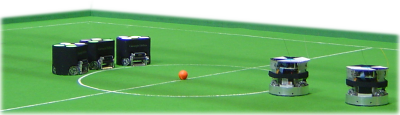
\includegraphics[scale=0.7]{./liga_robocup/F180}
	\caption{ Roboty biorące udział w \emph{Small-Size League}\newline(źródło: \texttt{www.robocup.org})} \label{fig:F180}
	\end{figure}
	
	\emph{Middle-size League} to rozgrywki w pełni autonomicznych robotów. W przeciwieństwie do poprzedniej ligi, globalny system wizyjny jest całkowicie zakazany.
	Każdy robot jest wyposażony w osobny zestaw czujników wizyjnych. Zawodnicy niezależnie muszą reagować na zmieniającą się sytuację na planszy oraz
	wspólnie dążyć do wypracowania wspólnej strategii w zależności od zachowań innych graczy.

	W projekcie wyróżnione są także ligi \emph{Standard Platform League }, czyli rozgrywki piesków \textit{Aibo} konstruowanych przez firmę \textit{Sony} oraz 
	liga robotów humanoidalnych. W tej ostatniej biorą udział roboty przypominające swoją budową ludzi czyli posiadające korpus, nogi, ręce oraz głowę.
	\section{Szczegółowe omówienie ligi Small-size (F180) \label{sec:F180}}
	\subsection{Zasady}
	Corocznie przed nowymi mistrzostwami wydawany jest zmodyfikowany regulamin, który będzie na nich obowiązywać. Zmiany nie są zazwyczaj daleko idące, modyfikacje dotyczą przykładowo nowego rozmiaru boiska.
	W poprzednich latach dopuszczono możliwość stosowania przez drużyny własnego globalnego systemu udostępniającego informację o położeniu i prędkości zawodników.
	Jednak od $2010$ roku sprawę systemu wizyjnego usystematyzowano, stworzono system o nazwie \textit{SSL-Vision}, który jest obowiązkowym w lidze. 
	Całkowity rozmiar boiska, wliczając w to pola autowe jest równy 7.4~[m] na 5.4~[m], natomiast sama plansza na której toczona jest rozgrywka ma wymiary 6.05~[m] na 4.05~[m].
	Powierzchnia jest równa i  wyłożona zielonym dywanem lub wykładziną. Podczas meczu wykorzystywana jest standardowa piłka do golfa koloru pomarańczowego. Jej promień jest równy 43~[mm], a masa
	46~[g].
	Uczestniczące drużyny mogą składać się z maksymalnie pięciu robotów, jeden z nich może zostać oddelegowany do pełnienia
	funkcji bramkarza, jednak powinno to zostać zgłoszone przed rozpoczęciem meczu. W trakcie rozgrywki roboty mogą być wymieniane na nowe, tak samo jak w rzeczywistym meczu, jednak 
	sytuacja taka musi być zgłoszona wcześniej arbitrowi.
	Konstrukcja mechaniczna robota nie jest mocno ograniczona, zalecenia dotyczą głównie wymiarów. Robot powinien zmieścić się w walcu o średnicy 18~[cm] oraz wysokości 15~[cm].
	Dodatkowo może on być wyposażony w urządzenie do prowadzenia piłki. Tutaj jednak istnieją pewne ograniczenia dotyczące
	samej budowy oraz stosowania w czasie gry. Zawodnik nie może pokonać z piłką odległości większej niż 50~[cm]. Po przejechaniu takiego dystansu powinien zdecydować się
	na podanie jej innemu zawodnikowi, oddanie strzału na bramkę lub kopnąć przed siebie i dalej z nia dryblować. Niedostosowanie się do tych zasad powoduje sygnalizowanie przez arbitra
	przewinienia i wykonanie rzutu wolnego przez drużynę przeciwną. Konstrukcja urządzenia do dryblowania nie powinna także uniemożliwiać kontaktu z piłką zawodnikowi z drużyny przeciwnej.
		
	Rozgrywka jest całkowicie kontrolowana przez arbitra, który czuwa nad tym, aby  regulamin był przestrzegany. Do
	jego zadań należy sygnalizowanie przewinień, zdobytych bramek oraz innych typowych sytuacji na boisku.
	Sędzia ma prawo zmienić swoją decyzje po konsultacjach z asystentem. Arbiter komunikuje się z zawodnikami za pomocą programu, którego interfejs użytkownika zamieszczono na rysunku \ref{fig:referee_box} .
	\begin{figure}[H]
	\centering
	\includegraphics[ scale=0.5]{./liga_robocup/referee_box}
	\caption{Program wykorzystywany przez sędziego w  \mbox{\emph{Small Size League}}\newline(źródło: \texttt{www.robocup.org}) }
	\label{fig:referee_box}
	\end{figure} 
	Wszystkie akcje sędziego wprowadzone do tego programu są udostępniane specjalnym protokołem zawodnikom, dzięki temu rozgrywka nie wymaga ludzkiej ingerencji.
	\subsection{Schemat komunikacji}
	Kluczową sprawą podczas rzeczywistej rozgrywki jest dostęp do informacji o położeniu piłki
	i pozostałych robotów. Jak już wspomniano wcześniej organizacja udostępnia drużynom system \textit{SSL-Vision}, z którego drużyny są zobowiązane pobierać te informacje. Uproszczony schemat systemu
	wizyjnego widoczny jest na rysunku~\ref{fig:comunication}.
	Składa się on z kamery ustawionej centralnie nad boiskiem oraz specjalnej aplikacji \mbox{\emph{SSL-Vision}}\footnote{ Do pobrania z \url{http://code.google.com/p/ssl-vision}}.
	Obecnie w skład systemu może wchodzić kilka kamer.
	Obraz zarejestrowany przez kamery jest przesyłany do komputera, gdzie jest przetwarzany przez \emph{SSL-Vision} w czasie rzeczywistym. Program dostarcza informację 
	o położeniu oraz prędkościach robotów i piłki. Dane te następnie są wykorzystywane przez rywalizujące ze sobą drużyny na potrzeby ich algorytmów sterujących zawodnikami.
 	Algorytm sterujący jako wynik swojego działania powinien zwracać kierunek i prędkość zawodników. Ta ostateczna informacja jest wysyłana droga radiową do zawodnika.
	\begin{figure}[H]
	\centering
	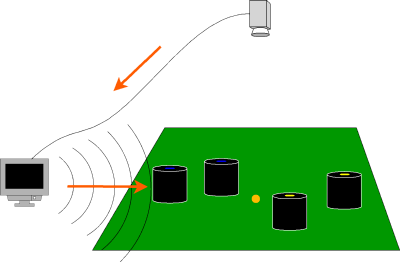
\includegraphics[ scale=0.5]{./liga_robocup/dataflow}
	\caption{Schemat komunikacji w  \mbox{\emph{Small Size League}}\newline(źródło: \texttt{www.robocup.org}) }
	\label{fig:comunication}
	\end{figure} 	
	\mbox{\emph{SSL-Vision}} może rozpoznawać nie tylko położenie poszczególnych robotów, ale także ich orientację na
	płaszczyźnie. Jednak do tego celu niezbędne jest zastosowanie specjalnych znaczników. Każdej z drużyn przed rozpoczęciem rozgrywki zostaje przypisana para kolorów,
	jakie zawiera znacznik. Dzięki zastosowaniu dwóch kolorów możliwe jest nie tylko rozróżnianie robotów z różnych drużyn, ale także określanie ich orientacji.

\section{Budowa robota \label{sec:budowa_robota} w \emph{Small-size League}}
	Oficjalne zasady ligi nie zobowiązują uczestników do używania konkretnych modeli robotów. Określone są jedynie rygory dotyczące maksymalnych wymiarów robota, oraz sposoby prowadzenia piłki.
	Obserwując kolejne mistrzostwa, łatwo zauważyć, że wśród zgłaszanych drużyn dominuje jedna konstrukcja mechaniczna. Została ona zaprezentowana na  rysunkach \ref{fig:F180_budowa}.
 	\begin{figure}
	\centering
	\subfloat[]{\label{fig:F180_budowa1}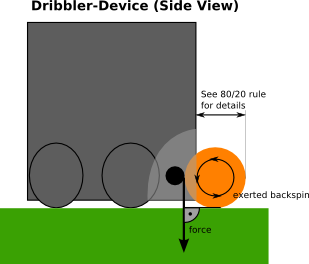
\includegraphics[ scale=0.34]{./liga_robocup/F180_budowa1}}
	\subfloat[]{\label{fig:F180_budowa2}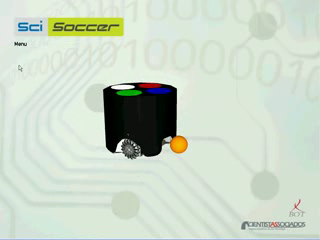
\includegraphics[ scale=0.38]{./liga_robocup/F180_budowa2}}
	\subfloat[]{\label{fig:F180_budowa3}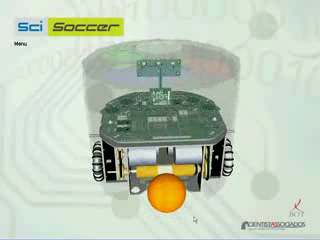
\includegraphics[ scale=0.38]{./liga_robocup/F180_budowa3}}
	\caption{Popularny model robota wykorzystywany w \mbox{lidze \emph{F180}}\newline(źródło: \texttt{www.robocup.org}) }
	\label{fig:F180_budowa}
	\end{figure}
	Podczas gry w piłkę nożną często wynika potrzeba zmiany orientacji w miejscu. W prezentowanym rozwiązaniu
	zdecydowano się na omnikierunkową bazę jezdną. Składa się ona z trzech kół szwedzkich, w tym dwóch niezależnie
	napędzanych. Koło szwedzkie posiada taką zaletę, iż dodatkowo poza obrotem wokół własnej osi umożliwia obrót
	wokół punktu styczności koła z podłożem oraz wokół osi rolek umieszczonych na kole.
	\begin{wrapfigure}{r}{0.42\textwidth}
	\vspace{-20pt}
	\begin{center}	
	\includegraphics[width=0.38\textwidth]{./liga_robocup/robocup_markers}
	\end{center}
	\caption{Znacznik umożliwiający systemowi wizyjnemu identyfikację robotów \newline(źródło: \texttt{www.robocup.org})\label{fig:znacznik}}
	\vspace{-60pt}
	\end{wrapfigure}
	Dzięki zastosowaniu takiego rozwiązania uzyskano w pełni holonomiczną budowę robota.
	Robot biorący udział w rozgrywkach musi być zdolny do prowadzenia piłki. Zastosowana konstrukcja jest wyposażona w urządzenie do dryblowania widoczne na rysunkach \ref{fig:F180_budowa1} oraz \ref{fig:F180_budowa3}. 
	Zbudowane jest ono z walca nadającego piłce wsteczną rotację, przez co nie odbija się ona od robota, a także nie traci on nad nią kontroli w momencie hamowania lub obracania się.
	
	W regulaminie rozgrywek dopuszczono do stosowania jedynie urządzenia do dryblowania działające na piłkę siłą prostopadłą do podłoża rys.~\ref{fig:F180_budowa1} (we wcześniejszych latach
	w użyciu były  urządzenia, w których obracany walec był umieszczony pionowo).

	Ostatnim ważnym elementem, w który musi być wyposażony robot, jest znacznik (rys.~\ref{fig:znacznik}).
	Znajduje się on w takim miejscu, aby kamera umieszczona centralnie nad boiskiem mogła go zarejestrować (przykrywa robota od góry).
	Znaczniki umożliwiają systemowi wizyjnemu określenie, do której drużyny należy dany robot, a także poprawne rozpoznanie jego pozycji, orientacji oraz prędkości
	na boisku.

